% Kept pitch deck (deliverable 7). Build: cd docs/deck && xelatex -jobname=Kept_pitch_deck deck.tex (twice)
\documentclass[aspectratio=169,10pt]{beamer}
\usepackage{fontspec}
\setsansfont{Carlito}
\usepackage{tikz}
\usetikzlibrary{positioning,arrows.meta,calc,fit,backgrounds}
\usepackage{booktabs}
\graphicspath{{../reports/figures/}}

\definecolor{kept}{HTML}{C8102E}
\definecolor{ink}{HTML}{1F2933}
\definecolor{muted}{HTML}{52606D}
\definecolor{edge}{HTML}{7B8794}
\definecolor{soft}{HTML}{F5F3EE}
\definecolor{kblue}{HTML}{2A78D6}
\definecolor{korange}{HTML}{E8833A}
\definecolor{kgreen}{HTML}{1BAF7A}
\setbeamercolor{normal text}{fg=ink,bg=white}
\setbeamercolor{frametitle}{fg=ink}
\setbeamercolor{structure}{fg=kept}
\setbeamerfont{frametitle}{size=\Large,series=\bfseries}
\setbeamertemplate{navigation symbols}{}
\setbeamertemplate{itemize items}{\color{kept}\textbullet}
\setbeamertemplate{frametitle}{\vspace{6pt}\insertframetitle\par\vspace{-2pt}{\color{kept}\rule{1.6cm}{2pt}}}
\setbeamertemplate{footline}{\hfill{\color{muted}\scriptsize Kept · Team Sharpe Shooters\quad\insertframenumber/\inserttotalframenumber}\hspace{8pt}\vspace{6pt}}
\newcommand{\stat}[3][4.2cm]{\begin{minipage}[t]{#1}\raggedright{\fontsize{22}{24}\selectfont\bfseries\color{kept}\mbox{#2}}\\[1pt]{\small\color{muted}#3}\end{minipage}}
\newcommand{\muted}[1]{{\color{muted}#1}}
\tikzset{
  b/.style={draw=edge, rounded corners=3pt, fill=white, align=center, font=\scriptsize, inner sep=3pt, text width=#1, minimum height=0.95cm},
  b/.default=2.1cm,
  hot/.style={draw=korange, line width=1pt},
  go/.style={-{Stealth[length=1.8mm]}, edge, line width=0.7pt},
}

\begin{document}

% ------------------------------------------------------------------ 1
\begin{frame}[plain]
\begin{tikzpicture}[remember picture, overlay]
\fill[soft] (current page.north west) rectangle (current page.south east);
\fill[kept] (current page.north west) rectangle ([xshift=0.35cm]current page.south west);
\end{tikzpicture}
\vspace{0.2cm}
{\fontsize{40}{42}\selectfont\bfseries Kept}\\[4pt]
{\Large A guarded next best action for promises customers can keep.}\\[22pt]
{\color{muted} Team Sharpe Shooters · CIBC Collections Hackathon · 4 Oct 2026}\\[4pt]
{\small\color{muted} Garimella Sai Abhishek · Satvik Rao · Shreyas Deb · Akshat Srivastava}\\[18pt]
\stat[3.4cm]{1.05M}{people, from 3.84M source keys}\hspace{0.2cm}\stat[3.2cm]{96,000}{guarded actions a night}\hspace{0.2cm}\stat[4.6cm]{62\% vs 52\%}{of promised money paid: payday-dated vs not}
\end{frame}

% ------------------------------------------------------------------ 2
\begin{frame}{The problem: generic treatment, promises set up to break}
\begin{columns}[T]
\column{0.5\textwidth}
\begin{itemize}\setlength\itemsep{6pt}
\item \textbf{One person, five IDs.} CRM, cards, loans, deposits and collections each key customers their own way. Agents see a slice.
\item \textbf{The facts are in free text.} ``Lost shifts at the plant, can pay 50 on the 15th'' lives in a note no system reads.
\item \textbf{Promises fall due before payday.} Same reminder, same day, for everyone. They break; the account rolls.
\item \textbf{Hardship found late.} Pressure on people who are already struggling, and regulator risk for the bank.
\end{itemize}
\column{0.46\textwidth}
\vspace{2pt}
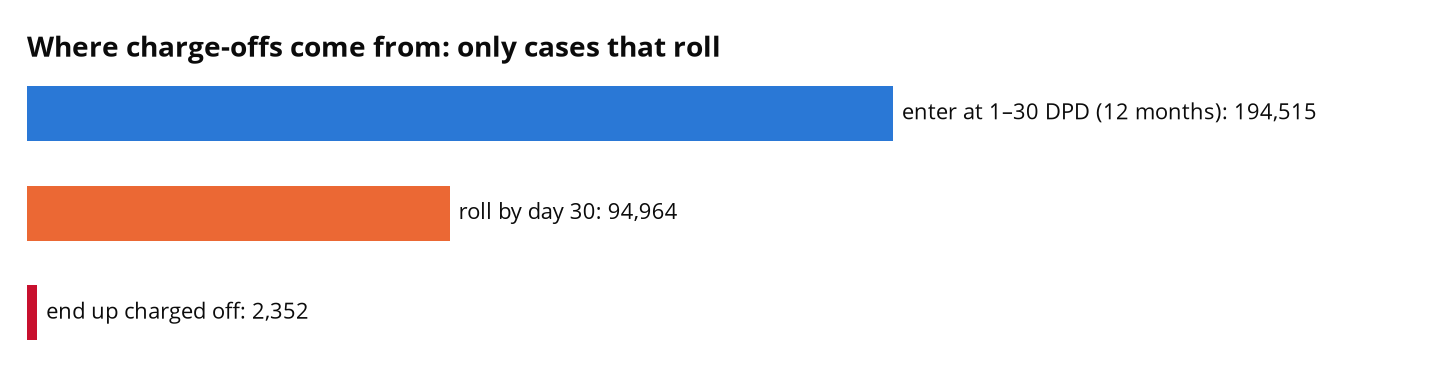
\includegraphics[width=\linewidth]{bc_funnel.png}\\[4pt]
{\small \textbf{48.8\%} of cases entering at 1–30 days past due roll by day 30. Rolling is the \emph{only} road to a charge-off: 2.5\% of rolled cases charge off (avg \$12.5K); 0\% of the rest.}
\end{columns}
\end{frame}

% ------------------------------------------------------------------ 3
\begin{frame}{The insight: when you ask matters as much as who you ask}
\begin{columns}[T]
\column{0.55\textwidth}
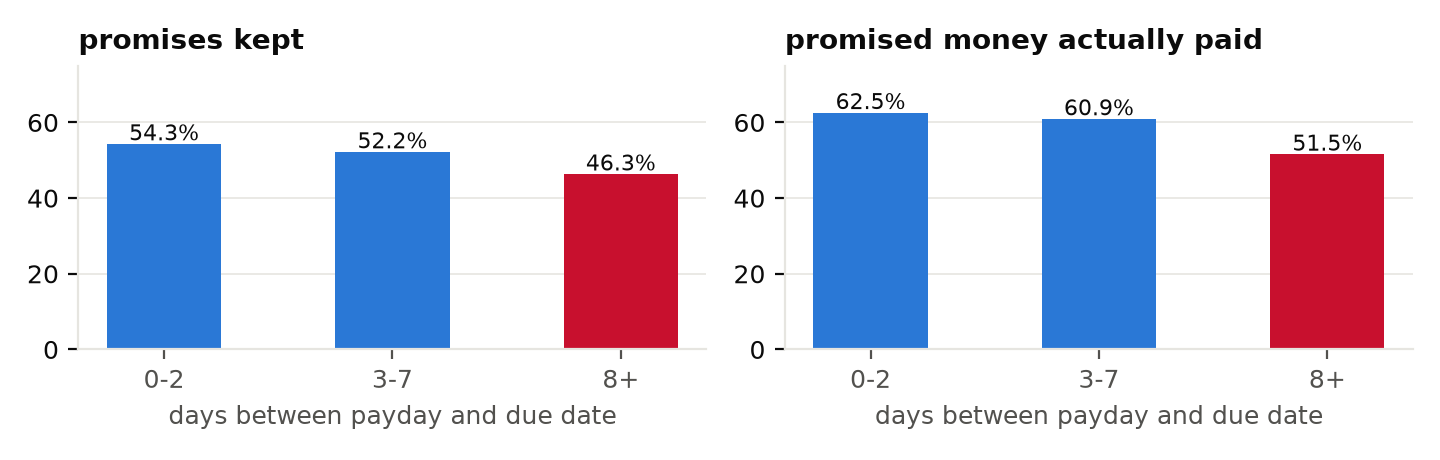
\includegraphics[width=\linewidth]{bc_payday.png}\\
{\small\muted{32,000 resolved promises where we can see the customer's salary deposits (bank's own history).}}
\column{0.42\textwidth}
\textbf{Kept = three ideas, in this order}
\begin{enumerate}\setlength\itemsep{5pt}
\item \textbf{Safety first.} Hard stops, consent, calling hours, contact caps and hardship are rules, not model outputs.
\item \textbf{Uplift, not ``likely to pay''.} Contact the people the action actually helps.
\item \textbf{Promises they can keep.} Due 1–2 days after payday, sized to spare cash.
\end{enumerate}
\vspace{4pt}
{\small A person releases every action.}
\end{columns}
\end{frame}

% ------------------------------------------------------------------ 4
\begin{frame}{The system: four layers, governance through all of them}
\centering
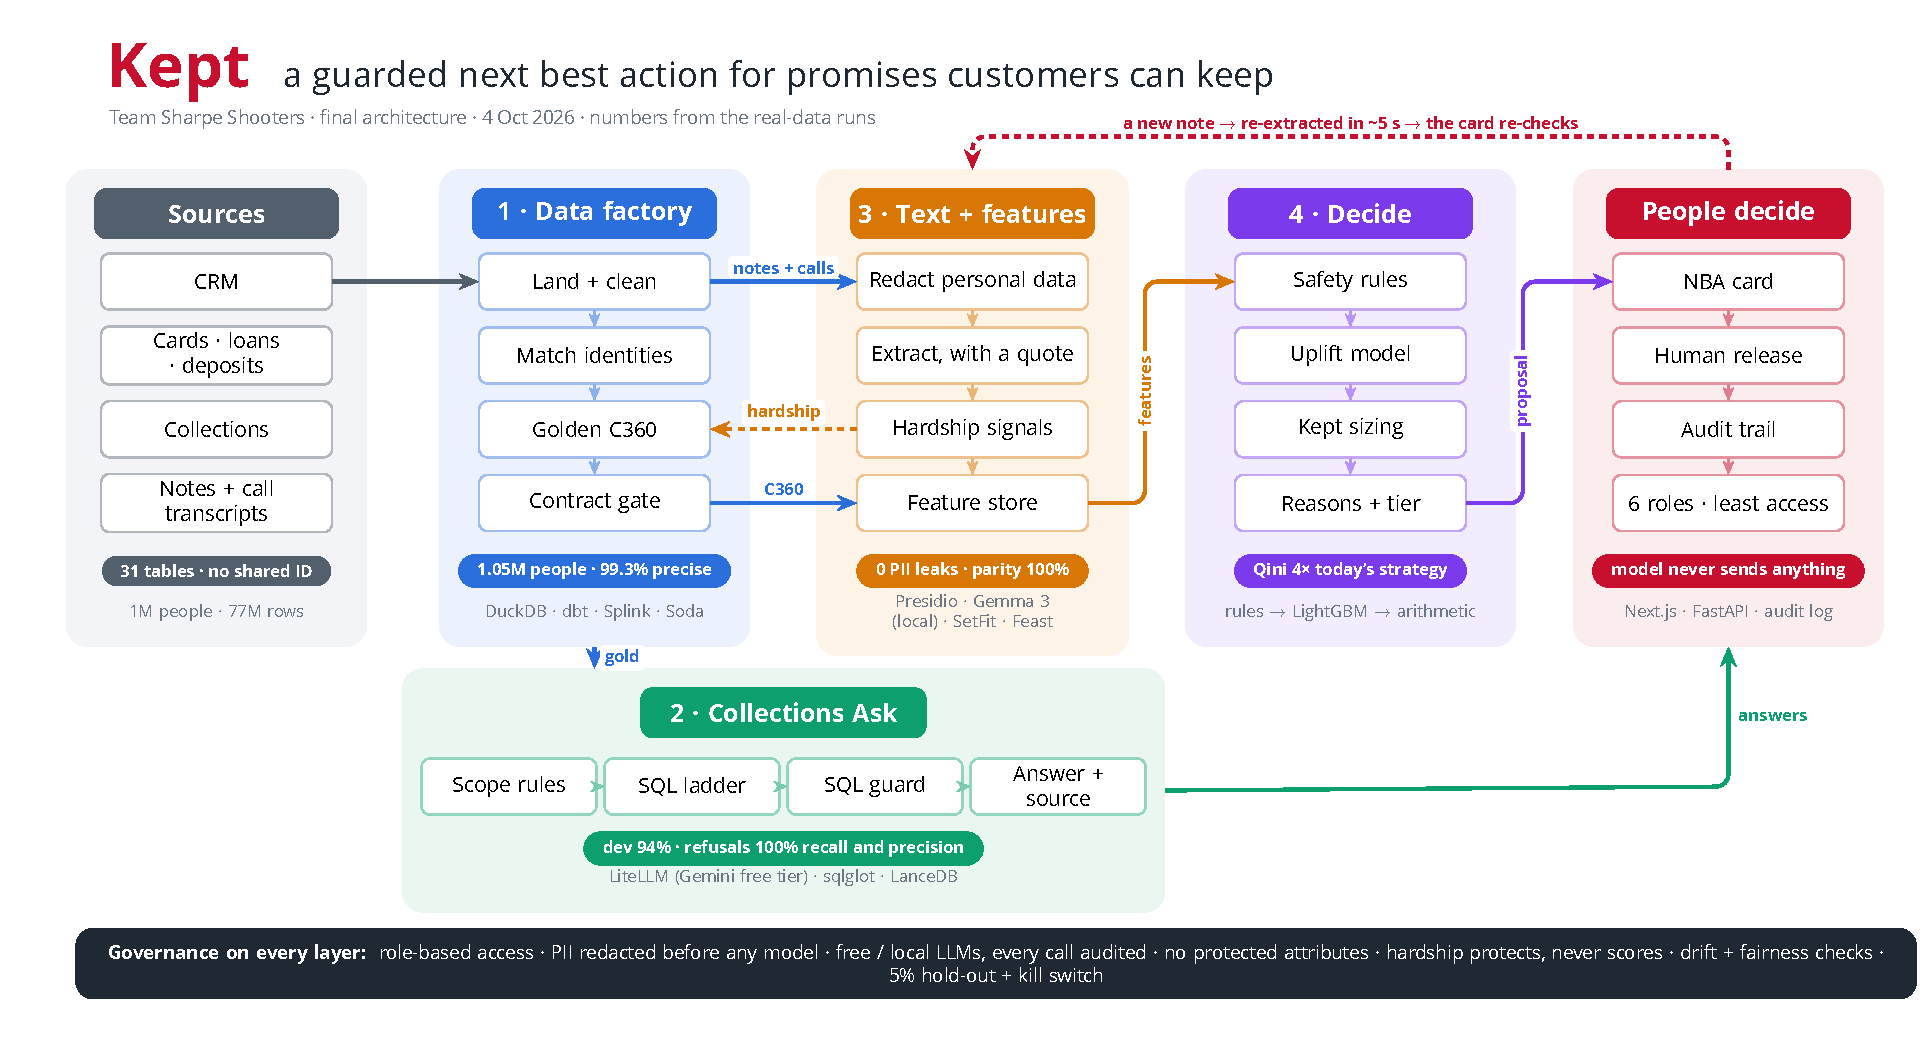
\includegraphics[width=\linewidth,height=0.78\textheight,keepaspectratio]{../architecture/architecture.pdf}\\[2pt]
{\scriptsize\color{muted} Full size: \texttt{docs/architecture/architecture.pdf}}
\end{frame}

% ------------------------------------------------------------------ 5
\begin{frame}{Layer 1 · one customer, one ID, a contract that blocks bad data}
\begin{columns}[T]
\column{0.48\textwidth}
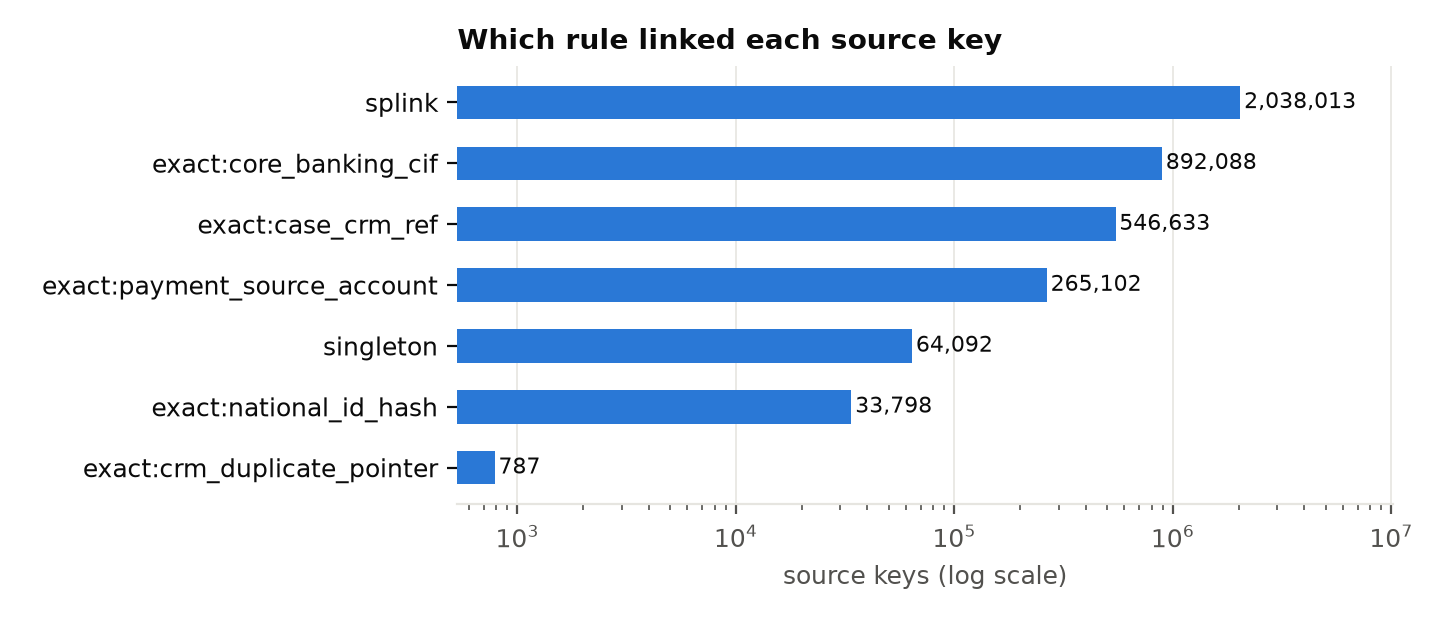
\includegraphics[width=\linewidth]{q_rules.png}\\[2pt]
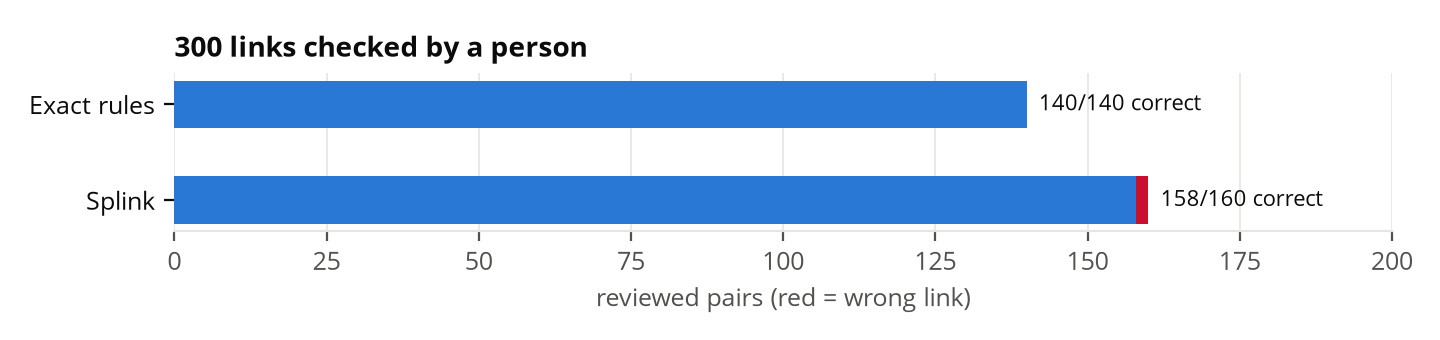
\includegraphics[width=\linewidth]{q_review.png}
\column{0.48\textwidth}
\stat[6.5cm]{3.84M → 1.05M}{source keys → golden IDs}\\[6pt]
\stat[6.5cm]{99.3\%}{match precision, 300 links checked by a person}\\[6pt]
\begin{itemize}\setlength\itemsep{3pt}\small
\item Exact keys, then Splink: ≥0.95 auto, 0.80–0.95 to a steward
\item \textbf{19 data traps} counted and handled; never guess
\item Contract from DC-COLL-001; gate \textbf{PASS}, all 8 rules
\end{itemize}
\end{columns}
\end{frame}

% ------------------------------------------------------------------ 6
\begin{frame}{Layer 2 · plain-English questions, answers with their working}
\centering
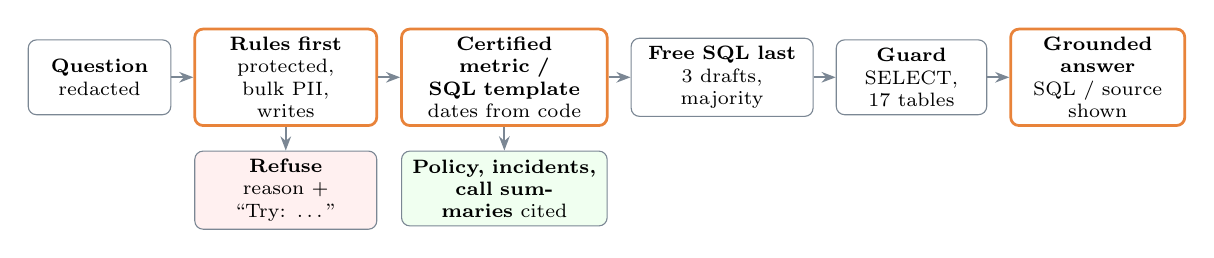
\begin{tikzpicture}[node distance=0.22cm and 0.28cm]
\node[b=1.6cm] (q) {\textbf{Question}\\ redacted};
\node[b, right=of q, hot] (r) {\textbf{Rules first}\\ protected, bulk PII,\\ writes};
\node[b=2.4cm, right=of r, hot] (c) {\textbf{Certified metric /}\\ \textbf{SQL template}\\ dates from code};
\node[b, right=of c] (fsql) {\textbf{Free SQL last}\\ 3 drafts, majority};
\node[b=1.7cm, right=of fsql] (g) {\textbf{Guard}\\ SELECT, 17 tables};
\node[b=2.0cm, right=of g, hot] (a) {\textbf{Grounded answer}\\ SQL / source shown};
\foreach \x/\y in {q/r, r/c, c/fsql, fsql/g, g/a} \draw[go] (\x) -- (\y);
\node[b, below=0.3cm of r, fill=red!6] (no) {\textbf{Refuse}\\ reason + ``Try: …''};
\node[b=2.4cm, below=0.3cm of c, fill=green!6] (d) {\textbf{Policy, incidents,}\\ \textbf{call summaries} cited};
\draw[go] (r) -- (no); \draw[go] (c) -- (d);
\end{tikzpicture}\\[10pt]
\stat{94\%}{dev accuracy (target 80\%)}\hspace{0.5cm}\stat{100\%}{refusal recall (target 95\%)}\hspace{0.5cm}\stat{100\%}{refusal precision}\\[8pt]
{\small Every number in an answer must appear in the result rows. Protected-attribute questions are refused \emph{before} any LLM sees them; close-sounding ones (``agents certified for vulnerable customers'') still get answered.}
\end{frame}

% ------------------------------------------------------------------ 7
\begin{frame}{Layer 3 · a note changes the action, in about five seconds}
\begin{columns}[T]
\column{0.52\textwidth}
\textbf{Live, on real data:}\\[4pt]
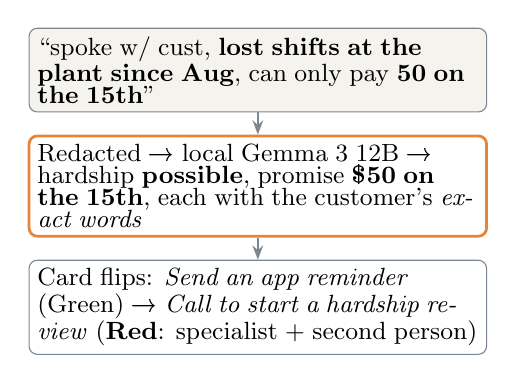
\begin{tikzpicture}[node distance=0.28cm]
\node[b=5.6cm, align=left, fill=soft] (n) {\small ``spoke w/ cust, \textbf{lost shifts at the plant since Aug}, can only pay \textbf{50 on the 15th}''};
\node[b=5.6cm, below=of n, hot, align=left] (x) {\small Redacted → local Gemma 3 12B → hardship \textbf{possible}, promise \textbf{\$50 on the 15th}, each with the customer's \emph{exact words}};
\node[b=5.6cm, below=of x, align=left] (c) {\small Card flips: \textit{Send an app reminder} (Green) → \textit{Call to start a hardship review} (\textbf{Red}: specialist + second person)};
\draw[go] (n) -- (x); \draw[go] (x) -- (c);
\end{tikzpicture}
\column{0.44\textwidth}
\stat[5.5cm]{0 leaks}{in 785,594 redacted notes and calls}\\[5pt]
\stat[5.5cm]{0.98 / 0.99}{hardship recall, notes / calls (held out)}\\[5pt]
\begin{itemize}\setlength\itemsep{2pt}\small
\item No quote, no value; text cease needs an agent
\item SetFit backfills 785K old texts in minutes
\item Cash-flow rule: late pay, pay cut, new EI
\item Feast: train = live (0 of 56,000 off)
\end{itemize}
\end{columns}
\end{frame}

% ------------------------------------------------------------------ 8
\begin{frame}{Layer 4 · the guarded next best action}
\centering
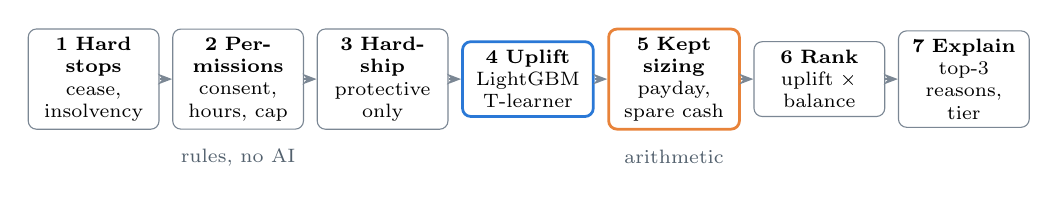
\begin{tikzpicture}[node distance=0.16cm]
\node[b=1.45cm] (s1) {\textbf{1 Hard stops}\\ cease, insolvency};
\node[b=1.45cm, right=of s1] (s2) {\textbf{2 Permissions}\\ consent, hours, cap};
\node[b=1.45cm, right=of s2] (s3) {\textbf{3 Hardship}\\ protective only};
\node[b=1.45cm, right=of s3, draw=kblue, line width=1pt] (s4) {\textbf{4 Uplift}\\ LightGBM T-learner};
\node[b=1.45cm, right=of s4, hot] (s5) {\textbf{5 Kept sizing}\\ payday, spare cash};
\node[b=1.45cm, right=of s5] (s6) {\textbf{6 Rank}\\ uplift × balance};
\node[b=1.45cm, right=of s6] (s7) {\textbf{7 Explain}\\ top-3 reasons, tier};
\foreach \x/\y in {s1/s2, s2/s3, s3/s4, s4/s5, s5/s6, s6/s7} \draw[go] (\x) -- (\y);
\node[font=\scriptsize, text=muted, below=0.12cm of s2] {rules, no AI};
\node[font=\scriptsize, text=muted, below=0.12cm of s5] {arithmetic};
\end{tikzpicture}\\[10pt]
\begin{columns}[T]
\column{0.5\textwidth}
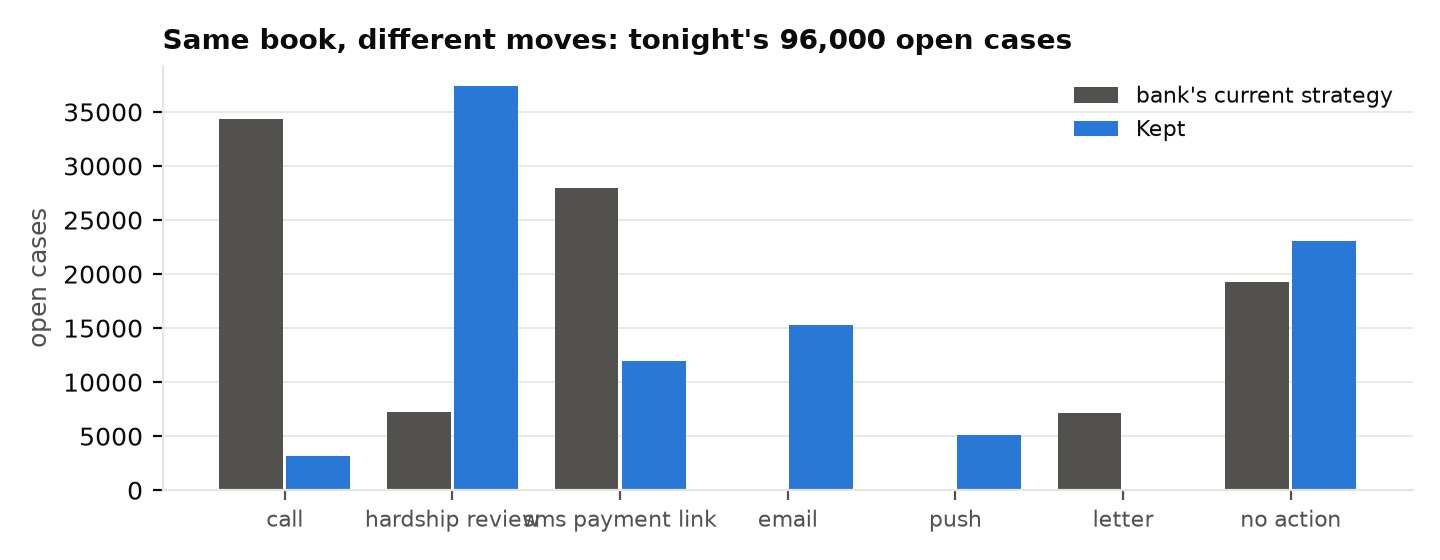
\includegraphics[width=\linewidth]{bc_mix.png}
\column{0.46\textwidth}
\stat[6.2cm]{+21 pts}{right-party contact for evening calls vs daytime calls (uplift study); contact itself barely moves payment}\\[8pt]
{\small Same number of calls as today, but 37K become \textbf{hardship reviews}; \$1.10 letters become near-free texts. Every card: three plain-English reasons, similar past cases, the checks that passed. Released by a person, re-checked at release.}
\end{columns}
\end{frame}

% ------------------------------------------------------------------ 9
\begin{frame}{Does it work, is it fair, what's it worth?}
\begin{columns}[T]
\column{0.5\textwidth}
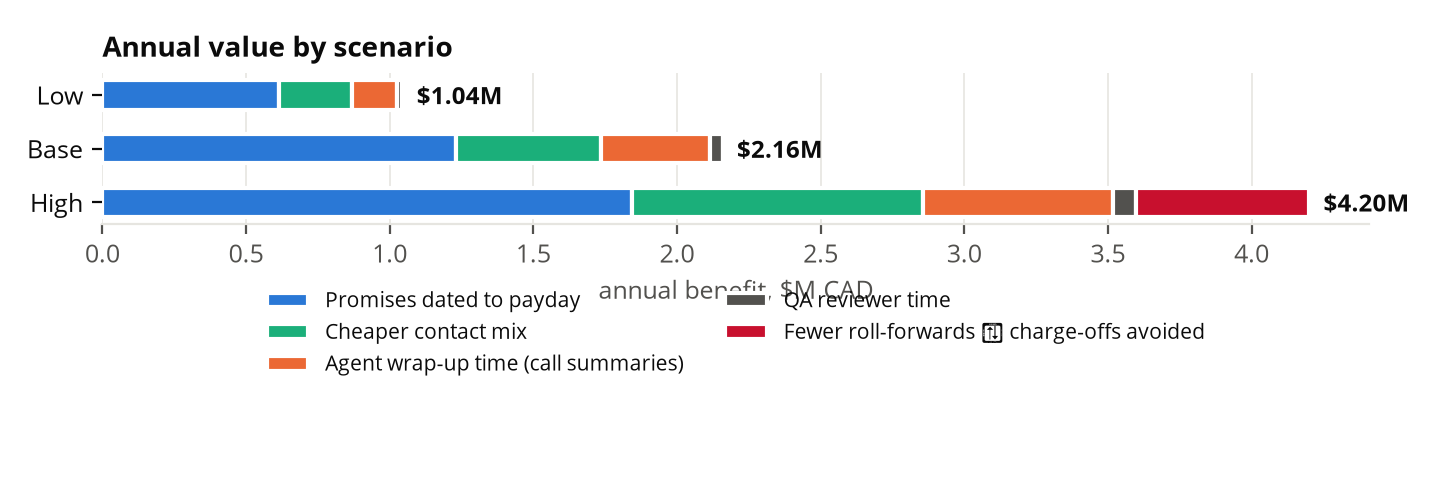
\includegraphics[width=\linewidth]{bc_scenarios.png}\\[2pt]
\stat[3.3cm]{\$2.2M/yr}{base case (\$1.0–4.2M)}\hspace{0.1cm}\stat[3.1cm]{3.8×}{year-1 ROI, payback \textasciitilde 2 mo}
\column{0.46\textwidth}
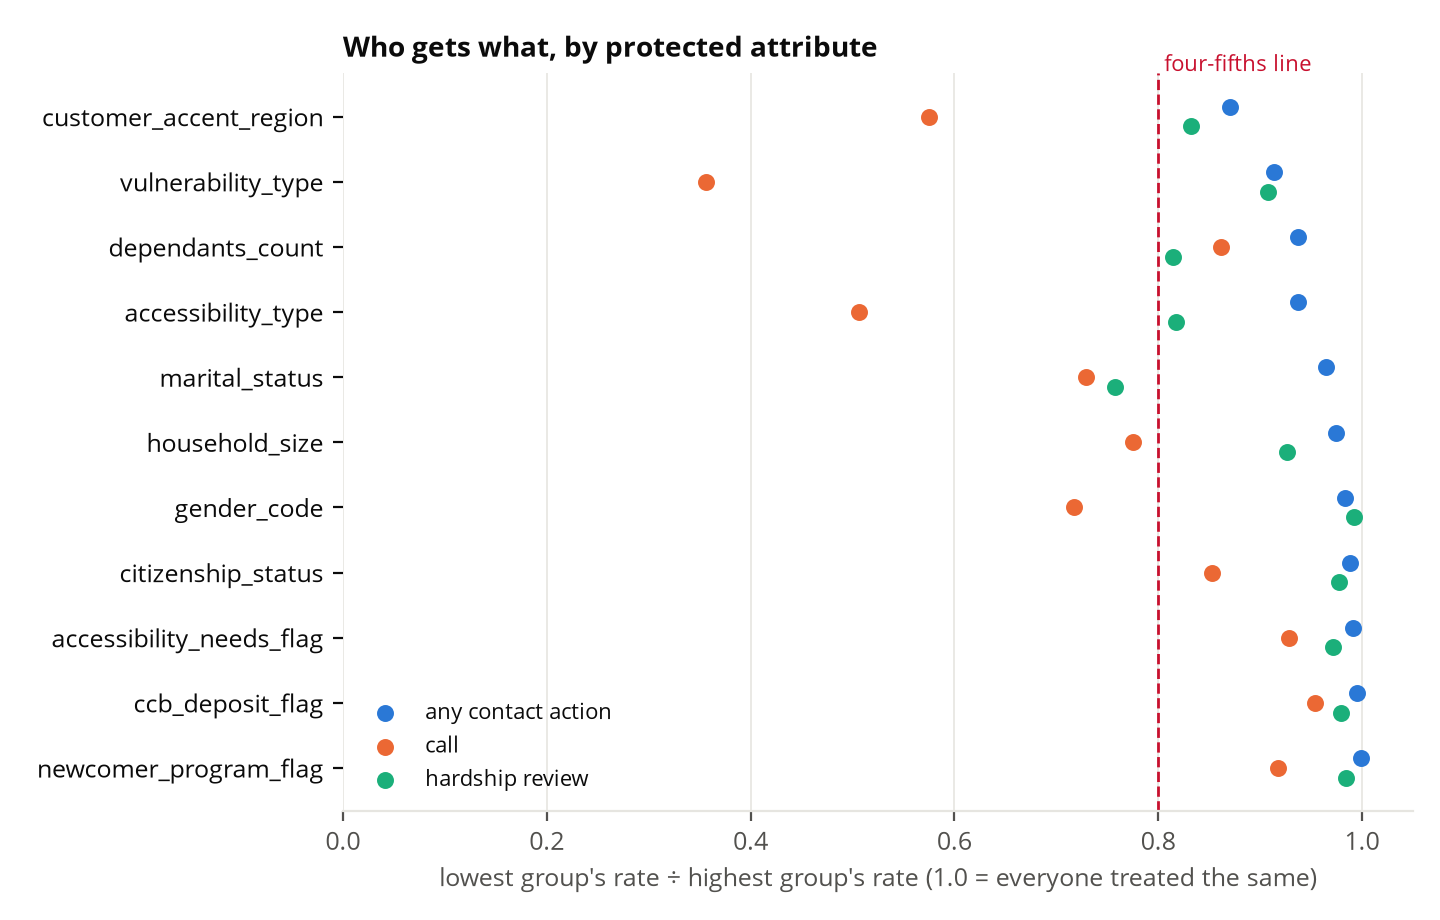
\includegraphics[width=\linewidth]{f_ratios.png}\\[2pt]
{\small \textbf{Fair:} any-contact rate within 0.86–1.00 across every protected group; flags only on rare calls and protective reviews.}\\[3pt]
{\small \textbf{Measured:} a 5\% hold-out stays on the old strategy; a kill switch reverts all.}
\end{columns}
\end{frame}

% ------------------------------------------------------------------ 10
\begin{frame}{Built responsibly, built together, and what's next}
\begin{columns}[T]
\column{0.32\textwidth}
\textbf{Responsible by construction}
\begin{itemize}\setlength\itemsep{2pt}\small
\item Human releases every action
\item Rules before and after the model
\item No protected attributes, tested
\item Redaction before any model
\item Free / local LLMs, all audited
\end{itemize}
\column{0.32\textwidth}
\textbf{Built together}
\begin{itemize}\setlength\itemsep{2pt}\small
\item 4 tracks: data · Ask · text · model + UI
\item Typed contracts between tracks, fakes for each
\item 5 integration gates (G0–G4)
\item 64 PRs · 315 commits · 1,200+ tests
\item One nightly: \textasciitilde 7 min, 1M people
\end{itemize}
\column{0.32\textwidth}
\textbf{Next}
\begin{itemize}\setlength\itemsep{2pt}\small
\item Retrain with payroll features (drift report found the gap)
\item Plan-aware rule to cut Red reviews
\item Score every call for QA with a fine-tuned fast classifier
\item Read the hold-out at day 30
\end{itemize}
\end{columns}
\vspace{14pt}
\centering{\Large\bfseries\color{kept} Promises customers can keep.}
\end{frame}

\end{document}
